\documentclass[tikz, border=1pt]{standalone}
\usepackage{tikz}
\usetikzlibrary{arrows.meta, positioning}
\usepackage{xcolor,colortbl}
% Define extra colors
\definecolor{darkgreen}{rgb}{0.0, 0.5, 0.0} % Define a darker green

\begin{document}


% \begin{figure}[h]
%     \centering

%     \begin{tikzpicture}[
%         claim/.style={rectangle, draw, rounded corners, align=center, text width=3.5cm, minimum height=1.5cm, fill=blue!20},
%         premise/.style={rectangle, draw, rounded corners, align=center, text width=3.5cm, minimum height=1.5cm, fill=yellow!50},
%         arrow/.style={-{Stealth}, thick},
%         support/.style={draw, -{Stealth}, thick, darkgreen},
%         attack/.style={draw, -{Stealth}, thick, red},
%         node distance=1cm and 1cm
%         ]

%         % Nodes
%         \node (claim1) [claim] {C1: Ce (L'Ukraine comme nation factice) n'est pas un thème neuf};
%         \node (claim2) [claim, below=of claim1] {C2: Vladimir Poutine a déjà cherché à reconstruire l'histoire ukrainienne et à nous offrir une interprétation très partiale de ce pays};
%         \node (claim5) [claim, right=of claim1, xshift=0.5cm] {C5: Vladimir Poutine veut le nier (la legitimite de l'Ukraine)};
%         \node (claim4) [claim, below=of claim5] {C4: Tous les états soviétiques, y compris la Russie, sont le produit de ces évènements historiques};
%         \node (claim3) [claim, right=of claim5, xshift=0.5cm] {C3: Tout discours sur l'historique de la construction nationale justifie nécessairement les objectifs du présent};
%         \node (premise1) [premise, below=of claim2] {P1: La propagande russe diffuse une carte géographique où l'Ukraine serait réduite à un petit centre};
%         \node (premise2) [premise, below=of premise1] {P2: Pour revenir à l'histoire de la construction nationale ukrainienne, cette carte n'évoque pas la période du début des années 1917-1918 où un Etat ukrainien indépendant, la République populaire d'Ukraine, se proclame en mars 1918};
%         \node (premise3) [premise, below=of claim4] {P3: Face à la création de cette nouvelle entité étatique, qui s'appuie sur une tradition à la fois intellectuelle et politique, et un travail de reconstruction d'une langue ukrainienne moderne à partir des patois, les bolchéviques sont obligés de créer eux aussi leur propre République socialiste d'Ukraine};
%         \node (premise4) [premise, right=of claim4, xshift=0.5cm] {P4: Toutes ces années de la guerre civile, les frontières sont mouvantes};
%         \node (premise5) [premise, below=of premise4] {P5: Il y a d'autres changements de territoire en amont et en aval de la Seconde Guerre Mondiale};

%         % Arrows with labels
%         \draw [support] (claim2) -- node[midway, right] {supports} (claim1);
%         \draw [support] (premise1) -- node[midway, right] {supports} (claim2);
%         \draw [support] (premise2) -- node[midway, right] {supports} (premise1);
%         \draw [support] (premise3) -- node[midway, right] {supports} (claim4);
%         \draw [support] (premise4) -- node[midway, above] {supports} (claim4);
%         \draw [support] (premise5) -- node[midway, right] {supports} (claim4);
%         \draw [support] (claim1) -- node[midway, above] {support} (claim5);
%         \draw [support] (claim3) -- node[midway, above] {support} (claim5);

%     \end{tikzpicture}
% \end{figure}

\begin{figure}
    \centering

    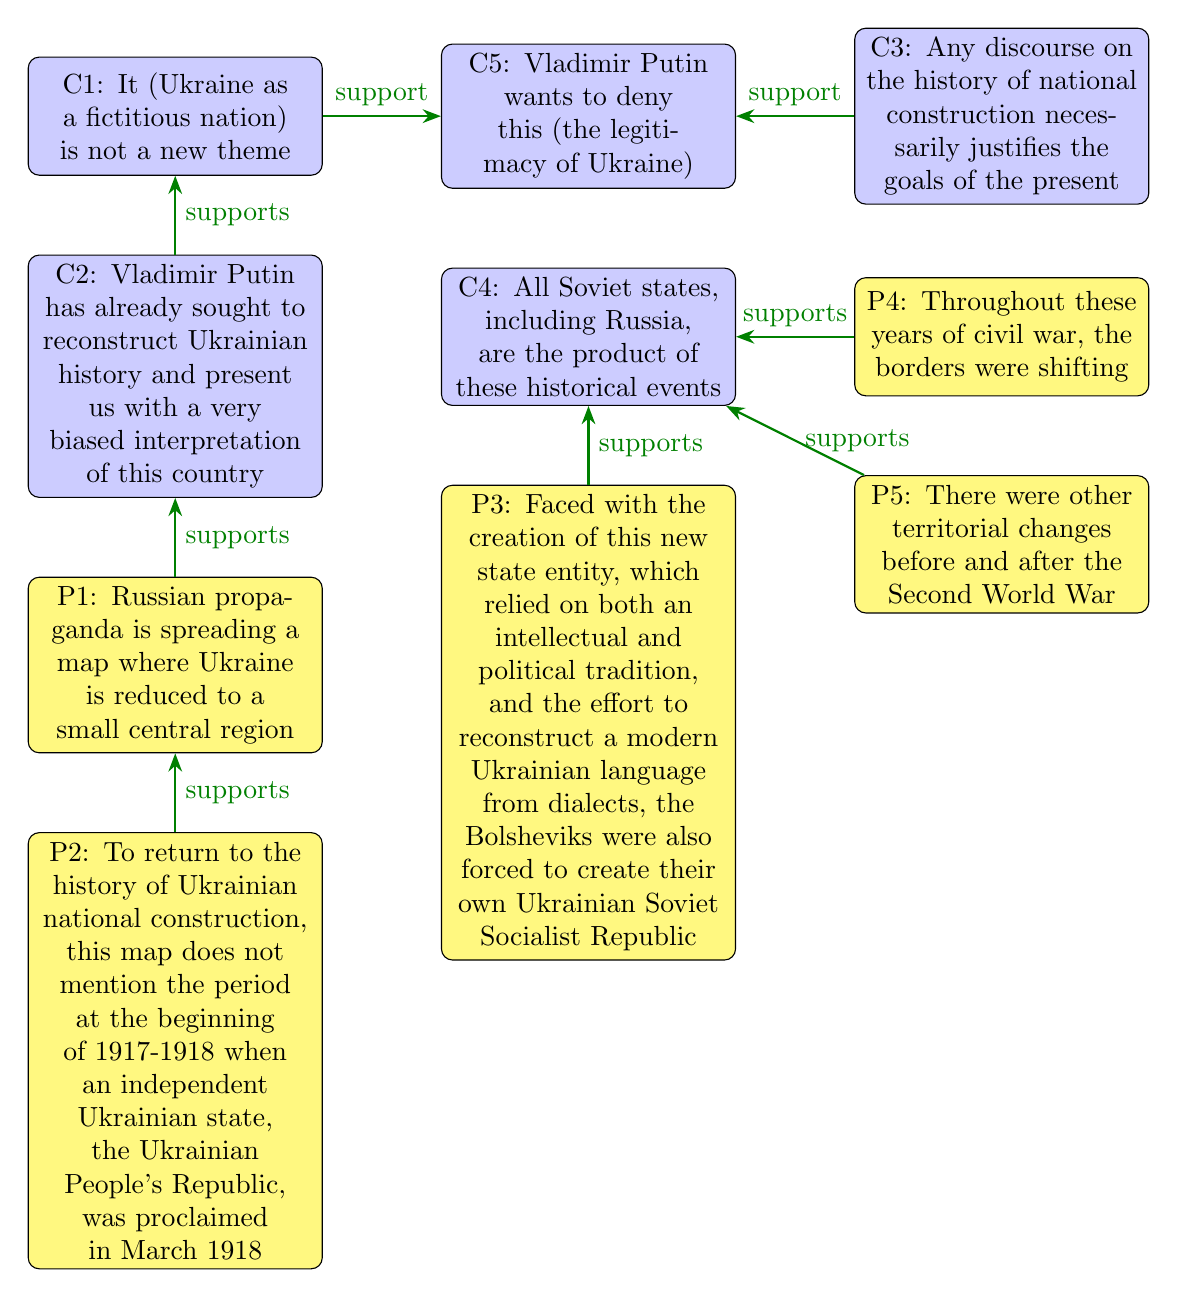
\begin{tikzpicture}[
        claim/.style={rectangle, draw, rounded corners, align=center, text width=3.5cm, minimum height=1.5cm, fill=blue!20},
        premise/.style={rectangle, draw, rounded corners, align=center, text width=3.5cm, minimum height=1.5cm, fill=yellow!50},
        arrow/.style={-{Stealth}, thick},
        support/.style={draw, -{Stealth}, thick, darkgreen},
        attack/.style={draw, -{Stealth}, thick, red},
        node distance=1cm and 1cm
        ]

        % Nodes
        \node (claim1) [claim] {C1: It (Ukraine as a fictitious nation) is not a new theme};
        \node (claim2) [claim, below=of claim1] {C2: Vladimir Putin has already sought to reconstruct Ukrainian history and present us with a very biased interpretation of this country};
        \node (claim5) [claim, right=of claim1, xshift=0.5cm] {C5: Vladimir Putin wants to deny this (the legitimacy of Ukraine)};
        \node (claim4) [claim, below=of claim5] {C4: All Soviet states, including Russia, are the product of these historical events};
        \node (claim3) [claim, right=of claim5, xshift=0.5cm] {C3: Any discourse on the history of national construction necessarily justifies the goals of the present};
        \node (premise1) [premise, below=of claim2] {P1: Russian propaganda is spreading a map where Ukraine is reduced to a small central region};
        \node (premise2) [premise, below=of premise1] {P2: To return to the history of Ukrainian national construction, this map does not mention the period at the beginning of 1917-1918 when an independent Ukrainian state, the Ukrainian People's Republic, was proclaimed in March 1918};
        \node (premise3) [premise, below=of claim4] {P3: Faced with the creation of this new state entity, which relied on both an intellectual and political tradition, and the effort to reconstruct a modern Ukrainian language from dialects, the Bolsheviks were also forced to create their own Ukrainian Soviet Socialist Republic};
        \node (premise4) [premise, right=of claim4, xshift=0.5cm] {P4: Throughout these years of civil war, the borders were shifting};
        \node (premise5) [premise, below=of premise4] {P5: There were other territorial changes before and after the Second World War};

        % Arrows with labels
        \draw [support] (claim2) -- node[midway, right] {supports} (claim1);
        \draw [support] (premise1) -- node[midway, right] {supports} (claim2);
        \draw [support] (premise2) -- node[midway, right] {supports} (premise1);
        \draw [support] (premise3) -- node[midway, right] {supports} (claim4);
        \draw [support] (premise4) -- node[midway, above] {supports} (claim4);
        \draw [support] (premise5) -- node[midway, right] {supports} (claim4);
        \draw [support] (claim1) -- node[midway, above] {support} (claim5);
        \draw [support] (claim3) -- node[midway, above] {support} (claim5);



    \end{tikzpicture}
    % \caption{Argumentation structure for Example \ref{ex:radiofrance}}
    \label{fig:radiofrance}
\end{figure}

\end{document}